\section{پروژه چهارم: تولید چهره با شبکه‌های زایای تخاصمی (\lr{DCGAN})}

در این پروژه، هدف ما طراحی و آموزش یک شبکه‌ی زایای تخاصمی عمیق (\lr{Deep Convolutional GAN}) برای تولید تصاویر چهره‌ی انسان است[cite: 6]. این شبکه‌ها از دو بخش اصلیِ مولد (\lr{Generator}) و متمایزکننده (\lr{Discriminator}) تشکیل شده‌اند که در یک بازیِ \lr{Minimax} با یکدیگر رقابت می‌کنند. طبق خواسته‌ی پروژه، پیاده‌سازی این مدل به‌طور کامل در فریم‌ورک \lr{Keras} انجام شده است[cite: 6].

\vspace{0.4cm}
\subsection{آماده‌سازی مجموعه‌داده‌ی \lr{CelebA}}

برای آموزش این شبکه از مجموعه‌داده‌ی معروف \lr{CelebA} استفاده کردیم که شامل بیش از ۲۰۰ هزار تصویر از چهره‌ی افراد مشهور است[cite: 6]. به دلیل حجم بالای داده‌ها، مدیریت حافظه در فرآیند آموزش اهمیت ویژه‌ای دارد.

\begin{stepbox}
\field{پیش‌پردازش داده‌ها و خط لوله (\lr{Data Pipeline})}{
\begin{itemize}
    \item \textbf{تغییر ابعاد:} تمامی تصاویر به ابعاد $64 \times 64$ پیکسل تغییر اندازه داده شدند تا شبکه‌ی ما بتواند با حفظ جزئیات کلی چهره، با سرعت و پایداری مناسبی آموزش ببیند.
    \item \textbf{نرمال‌سازی در بازه‌ی $[-1, 1]$:} از آنجا که لایه‌ی خروجی شبکه‌ی مولد ما از تابع فعال‌ساز \lr{Tanh} استفاده خواهد کرد، مقادیر پیکسل‌های تصاویر واقعی را از بازه‌ی $[0, 255]$ به $[-1, 1]$ انتقال دادیم.
    \item \textbf{خط لوله‌ی \lr{tf.data}:} برای تزریق سریع و بهینه‌ی داده‌ها به گراف محاسباتی، از \lr{tf.data.Dataset} با اندازه‌ی دسته‌ی (\lr{Batch Size}) برابر با ۱۲۸ استفاده شد.
\end{itemize}
}
\end{stepbox}

\begin{figure}[h!]
    \centering
    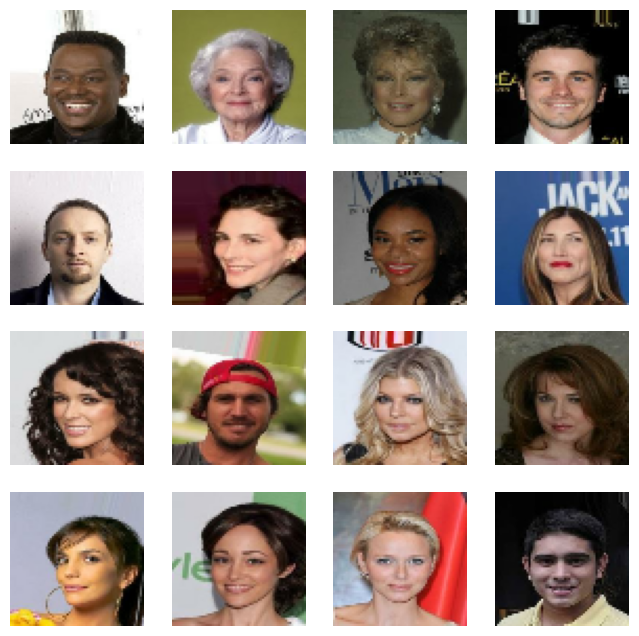
\includegraphics[width=0.75\textwidth]{images/celeba_samples.png}
    \caption{نمونه‌هایی از تصاویر واقعی چهره در مجموعه‌داده‌ی \lr{CelebA} پس از تغییر ابعاد به $64 \times 64$}
    \label{fig:celeba_samples}
\end{figure}

\vspace{0.4cm}
\subsection{طراحی معماری \lr{DCGAN}}

در این بخش، معماری دو شبکه‌ی مولد (\lr{Generator}) و متمایزکننده (\lr{Discriminator}) را بر اساس استانداردهای \lr{DCGAN} پیاده‌سازی کردیم. 

\begin{stepbox}
\field{شبکه‌ی مولد (\lr{Generator})}{
وظیفه‌ی این شبکه، تبدیل یک بردار نویز تصادفی ۱۰۰ بُعدی (فضای نهان) به یک تصویر با ابعاد $64 \times 64 \times 3$ است. برای این منظور ابتدا نویز ورودی توسط یک لایه‌ی متراکم (\lr{Dense}) به یک نقشه‌ی ویژگی ۸ در ۸ تبدیل شده و سپس با استفاده از سه لایه‌ی کانولوشن ترانهاده (\lr{Conv2DTranspose})، ابعاد تصویر به صورت پله‌پله افزایش می‌یابد. در لایه‌های میانی از فعال‌ساز \lr{LeakyReLU} و \lr{BatchNormalization} استفاده کردیم. لایه‌ی خروجی نیز با فعال‌ساز \lr{Tanh} تنظیم شد تا خروجی‌ها در بازه‌ی $[-1, 1]$ قرار گیرند. طبق بررسی‌ها، این شبکه دارای \textbf{$2,733,504$} پارامتر می‌باشد.
}
\vspace{0.2cm}
\newpage
\field{شبکه‌ی متمایزکننده (\lr{Discriminator})}{
این شبکه یک دسته‌بند دودویی است که تصویر را به عنوان ورودی دریافت کرده و با استفاده از لایه‌های کانولوشنال (\lr{Conv2D}) به همراه \lr{LeakyReLU} و \lr{Dropout} (جهت کنترل بیش‌برازش)، ابعاد فضایی تصویر را کاهش داده و ویژگی‌های آن را استخراج می‌کند. در نهایت یک لایه‌ی متراکم با یک نورون خام (\lr{Logit}) واقعی یا جعلی بودن تصویر را تخمین می‌زند. این شبکه در مجموع دارای \textbf{$1,045,633$} پارامتر قابل آموزش است.
}
\end{stepbox}

\vspace{0.4cm}
\subsection{حلقه‌ی آموزش، چالش‌های پردازشی و تولید خروجی}

آموزش شبکه‌های \lr{GAN} به دلیل ساختار دوگانه‌ی آن‌ها، نیازمند یک حلقه‌ی آموزش سفارشی است و نمی‌توان از متدهای معمول مانند \lr{model.fit} استفاده کرد. ما این حلقه را با استفاده از \lr{tf.GradientTape} پیاده‌سازی کردیم تا گرادیان‌های هر شبکه به‌صورت مستقل محاسبه و به‌روزرسانی شوند. 

\begin{stepbox}
\field{مدیریت منابع و بهینه‌سازی سرعت آموزش}{
\begin{itemize}
    \item \textbf{سیستم بازیابی (\lr{Checkpoint}):} با توجه به زمان‌بر بودن آموزش روی \lr{Google Colab} و احتمال قطع شدن ارتباط، از کلاس \lr{tf.train.Checkpoint} استفاده کردیم تا وضعیت بهینه‌سازها و وزن‌های مدل در هر اپوک ذخیره شود.
    \item \textbf{بخش‌بندی داده‌ها و کَش (\lr{Caching}):} مجموعه‌داده‌ی \lr{CelebA} بسیار حجیم است. برای جلوگیری از افت شدید سرعت، آموزش را به زیرمجموعه‌ای شامل ۵۰ هزار تصویر محدود کردیم و با استفاده از متد \lr{.cache()} در خط لوله‌ی \lr{tf.data}، تصاویر را در حافظه‌ی موقت (\lr{RAM}) سیستم بارگذاری کردیم که این کار سرعت پردازش هر اپوک را به‌طور چشم‌گیری افزایش داد.
\end{itemize}
}
\end{stepbox}

\vspace{0.3cm}
\subsection{تحلیل نتایج نهایی و روند آموزش}

از آنجا که فرمت \lr{PDF} به‌صورت استاندارد از تصاویر متحرک پشتیبانی نمی‌کند، برای نمایش دقیق روند پیشرفت شبکه، خروجی‌های مدل مولد را در پایان هر اپوک به‌صورت فریم‌های مجزا استخراج کردیم. فایل انیمیشن (\lr{GIF}) نهایی که در صورت‌پروژه خواسته شده بود[cite: 6]، ساخته شده و به همراه کدهای اصلی در مخزن گیت‌هاب پروژه قرار گرفته است.

شکل \ref{fig:gan_progression} وضعیت چهره‌های تولید شده از یک بردار نویز ثابت را در طول ۵ اپوک متوالی نشان می‌دهد.

\begin{figure}[h!]
    \centering
    \begin{subfigure}{0.19\textwidth}
        \centering
        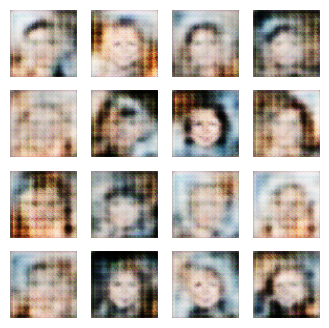
\includegraphics[width=\textwidth]{images/image_at_epoch_0001.png}
        \caption{اپوک ۱}
    \end{subfigure}
    \hfill
    \begin{subfigure}{0.19\textwidth}
        \centering
        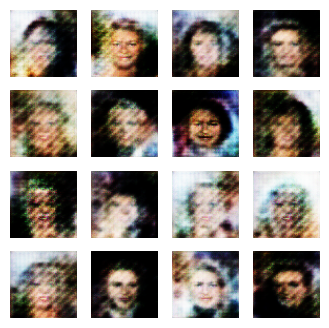
\includegraphics[width=\textwidth]{images/image_at_epoch_0002.png}
        \caption{اپوک ۲}
    \end{subfigure}
    \hfill
    \begin{subfigure}{0.19\textwidth}
        \centering
        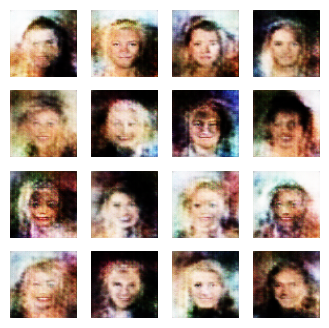
\includegraphics[width=\textwidth]{images/image_at_epoch_0003.png}
        \caption{اپوک ۳}
    \end{subfigure}
    \hfill
    \begin{subfigure}{0.19\textwidth}
        \centering
        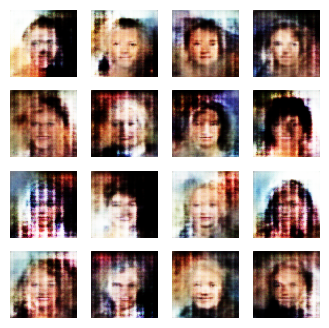
\includegraphics[width=\textwidth]{images/image_at_epoch_0004.png}
        \caption{اپوک ۴}
    \end{subfigure}
    \hfill
    \begin{subfigure}{0.19\textwidth}
        \centering
        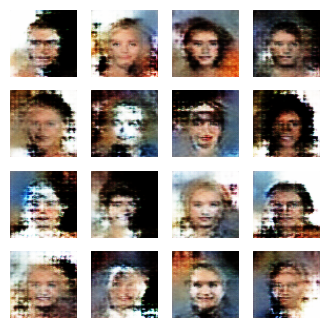
\includegraphics[width=\textwidth]{images/image_at_epoch_0005.png}
        \caption{اپوک ۵}
    \end{subfigure}
    \caption{روند آموزش و تولید چهره توسط شبکه‌ی \lr{DCGAN} در طول ۵ اپوک متوالی. تکامل ساختار چهره و کاهش نویزها در هر مرحله مشهود است.}
    \label{fig:gan_progression}
\end{figure}

\begin{notebox}[بررسی کیفیت تصاویر تولید شده]
با بررسی فریم‌به‌فریم تصاویر در شکل \ref{fig:gan_progression}، روند یادگیری شبکه کاملاً مشخص است. در اپوک اول، خروجی‌ها بیشتر شامل نویز و الگوهای شطرنجی (\lr{Checkerboard Artifacts}) هستند. اما با پیشروی به سمت اپوک پنجم، شبکه‌ی مولد توانسته است توزیع مکانیِ ساختار چهره را به‌خوبی درک کند. تناسبات پایه‌ای مانند محل قرارگیری چشم‌ها، فرم سر، رنگ پوست و تمایز پس‌زمینه در اکثر تصاویر اپوک پنجم شکل گرفته‌اند. با توجه به محدودیت شدید در تعداد اپوک‌ها (برای مدیریت زمان پردازش)، رسیدن از نویز مطلق به این سطح از درک ساختاری، نشان‌دهنده‌ی معماری درست و روند کاملاً صحیح آموزش مدل است.
\end{notebox}

\begin{warnbox}[چالش‌های سخت‌افزاری و استدلال محدودیت آموزش به ۵ اپوک]
آموزش شبکه‌های زایای تخاصمی (\lr{GAN}) ذاتاً فرآیندی بسیار زمان‌بر و نیازمند منابع محاسباتی عظیم است. با توجه به حجم بالای مجموعه‌داده‌ی \lr{CelebA} و پیچیدگی گراف محاسباتی در به‌روزرسانی‌های همزمان شبکه‌های مولد و متمایزکننده در فریم‌ورک \lr{Keras}، اجرای طولانی‌مدت مدل در محیط‌های ابری اشتراکی نظیر \lr{Google Colab} با محدودیت‌های جدی مواجه است. 

خطر قطعی ناگهانی اتصال (\lr{Runtime Disconnection})، محدودیت حافظه‌ی \lr{RAM} و سقف زمانی استفاده از پردازنده‌های گرافیکی (\lr{GPU}) رایگان، از مهم‌ترین چالش‌های پردازشی این مرحله بودند. به همین دلیل، از منظر مهندسی و آکادمیک تصمیم بر آن شد تا آموزش مدل روی یک زیرمجموعه‌ی هدفمند و تنها برای ۵ اپوک انجام شود. 

هدف از این پیکربندی، رسیدن به همگرایی مطلق و تولید چهره‌های بی‌نقصِ واقع‌گرایانه (که نیازمند چندین روز پردازش مداوم بر روی سخت‌افزارهای تجاری است) نبود؛ بلکه هدف اصلی اثبات صحت پیاده‌سازی معماری \lr{DCGAN}، عملکرد صحیح توابع زیان و مشاهده‌ی روند تکامل الگوها از نویز خالص به ساختار پایه‌ی چهره بود که این مهم به‌طور کامل و موفقیت‌آمیز در نتایج خروجی محقق گردید.
\end{warnbox}